% coding:utf-8

%FOSAET, a LaTeX-Code for a electrical summary of basic electronics
%Copyright (C) 2013, Daniel Winz, Ervin Mazlagic

%This program is free software; you can redistribute it and/or
%modify it under the terms of the GNU General Public License
%as published by the Free Software Foundation; either version 2
%of the License, or (at your option) any later version.

%This program is distributed in the hope that it will be useful,
%but WITHOUT ANY WARRANTY; without even the implied warranty of
%MERCHANTABILITY or FITNESS FOR A PARTICULAR PURPOSE.  See the
%GNU General Public License for more details.
%----------------------------------------

\section{Komplexe Impedanz}

\subsubsection{Widerstand}
\[ Z_R = R \]
\[ u_R = R \cdot i_R \]
\begin{figure}[h!]
	\centering
	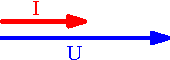
\includegraphics[width=0.3\textwidth]{zeig_ui_wid.pdf}
	\caption{Zeigerdiagramm Widerstand}
	\label{fig:zeig_ui_wid}
\end{figure}

\newpage
\subsubsection{Kondensator}
\[ Z_C = \frac{1}{j \cdot \omega \cdot C} 
= \frac{1}{j \cdot 2 \cdot \pi \cdot f \cdot C} \]
\[ x_C = Im(Z_C) = -\frac{1}{\omega \cdot C} 
= -\frac{1}{2 \cdot \pi \cdot f \cdot C} \]
\[ u_C = \left( \frac{1}{C} \cdot \int i_C ~ dt \right) + U_C(0) \]
\[ i_C = C \cdot \frac{du_C}{dt} \]
\begin{figure}[h!]
	\centering
	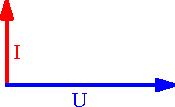
\includegraphics[width=0.3\textwidth]{zeig_ui_kap.pdf}
	\caption{Zeigerdiagramm Kondensator}
	\label{fig:zeig_ui_kap}
\end{figure}

\subsubsection{Spule}
\[ Z_L = j \cdot \omega \cdot L = j \cdot 2 \cdot \pi \cdot f \cdot L \]
\[ x_L = Im(Z_L) = \omega \cdot L = 2 \cdot \pi \cdot f \cdot L \]
\[ u_L = L \cdot \frac{di_L}{dt} \]
\[ i_L = \left( \frac{1}{L} \cdot \int u_L ~ dt \right) + I_L(0) \]
\begin{figure}[h!]
	\centering
	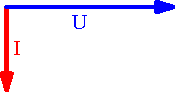
\includegraphics[width=0.3\textwidth]{zeig_ui_ind.pdf}
	\caption{Zeigerdiagramm Spule}
	\label{fig:zeig_ui_ind}
\end{figure}
